\documentclass[border=12pt]{standalone}
\def\pgfsysdriver{pgfsys-dvisvgm.def}
\usepackage[dvisvgm]{xcolor}
\usepackage{xeCJK}
\setCJKmainfont{HaranoAjiGothic-Regular.otf}[BoldFont=HaranoAjiGothic-Bold.otf]
\setCJKsansfont{HaranoAjiGothic-Regular.otf}[BoldFont=HaranoAjiGothic-Bold.otf]
\usepackage{amsmath,amssymb,tikz,lmodern}
\usetikzlibrary{arrows.meta,positioning,calc,fit,backgrounds}
\renewcommand{\familydefault}{\sfdefault}
\definecolor{ink}{HTML}{25322F}
\definecolor{green}{HTML}{246657}
\definecolor{tint}{HTML}{EEF4F0}
\definecolor{soft}{HTML}{C6D2CC}
\definecolor{muted}{HTML}{52615B}
\newif\ifJapanese
\newcommand{\Tx}[2]{\ifJapanese #1\else #2\fi}
\newcommand{\Eff}{\overline{\operatorname{Eff}}}
\newcommand{\heading}[3]{{\color{green}\bfseries #1\quad\Tx{#2}{#3}}\\[5pt]}
% A white rectangle makes the complete citation label clickable, including spaces.
\newcommand{\refurl}[2]{\special{dvisvgm:raw <a xlink:href="#1" target="_blank" rel="noopener noreferrer">}{\setlength{\fboxsep}{0pt}\colorbox{white}{\color{green}\underline{\strut #2}}}\special{dvisvgm:raw </a>}}
\newcommand{\refedge}[3]{\refurl{\csname source#1\endcsname\string##page=#2}{#3}}
\newcommand{\SF}[2]{\refedge{sf}{#1}{#2}}
% GitHub's file preview does not support PDF page fragments.
\newcommand{\LA}[2]{\refurl{\sourcela}{#2}}
\newcommand{\Sch}[2]{\refedge{sch}{#1}{#2}}
\newcommand{\PS}[2]{\refedge{ps}{#1}{#2}}
\tikzset{
 card/.style={draw=soft,fill=white,rounded corners=2pt,align=left,text=ink,font=\fontsize{10.5}{14}\selectfont,inner xsep=12pt,inner ysep=10pt,text width=14.4cm},
 half/.style={card,text width=6.45cm,minimum height=2.05cm},
 result/.style={card,draw=green,fill=tint,line width=.9pt},
 reason/.style={align=left,text=muted,font=\fontsize{9}{12}\selectfont,inner sep=0pt,text width=12.7cm},
 branchreason/.style={reason,text width=5.95cm},
 edge/.style={-{Stealth[length=2.4mm]},draw=green,line width=1pt},
 wire/.style={draw=green,line width=1pt},
}
% Keep the arrow in a dedicated left gutter; explanations never cover it.
\newcommand{\flow}[3]{
 \coordinate (#2-from) at ($(#1.south)+(-6.9,0)$);
 \coordinate (#2-to) at ($(#2.north)+(-6.9,0)$);
 \draw[edge] (#2-from)--(#2-to);
 \node[reason,anchor=west] (#2-reason) at ($(#2-from)!.5!(#2-to)+(.55,0)$) {#3};
}


\newcommand{\CiteSource}[2]{\refurl{\csname source#1\endcsname}{#2}}

\expandafter\def\csname sourceS\endcsname{https://github.com/openai/math/blob/adc7f1241b42e322a6451854ab7e4b4c146bf78a/preprints/Lifting-sections-from-the-reduced-support-of-an-adjoint-September-27-2026/paper.pdf}
\expandafter\def\csname sourceNV\endcsname{https://github.com/openai/math/blob/adc7f1241b42e322a6451854ab7e4b4c146bf78a/preprints/Fourfold-nonvanishing-by-minimal-metrics-and-moving-jets-September-27-2026/paper.pdf}
\expandafter\def\csname sourceFG\endcsname{https://www.math.kyoto-u.ac.jp/~fujino/fg-comp-final.pdf}
\expandafter\def\csname sourceKS\endcsname{https://people.math.harvard.edu/~mpopa/papers/oxford.pdf}
\expandafter\def\csname sourceHash\endcsname{https://arxiv.org/html/1609.00121v4}
\expandafter\def\csname sourceBir\endcsname{https://arxiv.org/pdf/0706.1792}
\expandafter\def\csname sourceSaito\endcsname{https://doi.org/10.2977/PRIMS/1195171082}
\expandafter\def\csname sourceUfour\endcsname{https://github.com/openai/math/blob/adc7f1241b42e322a6451854ab7e4b4c146bf78a/preprints/Uniform-effective-log-Iitaka-fibrations-for-fourfolds-September-26-2026/paper.pdf}

\Japanesetrue
\begin{document}
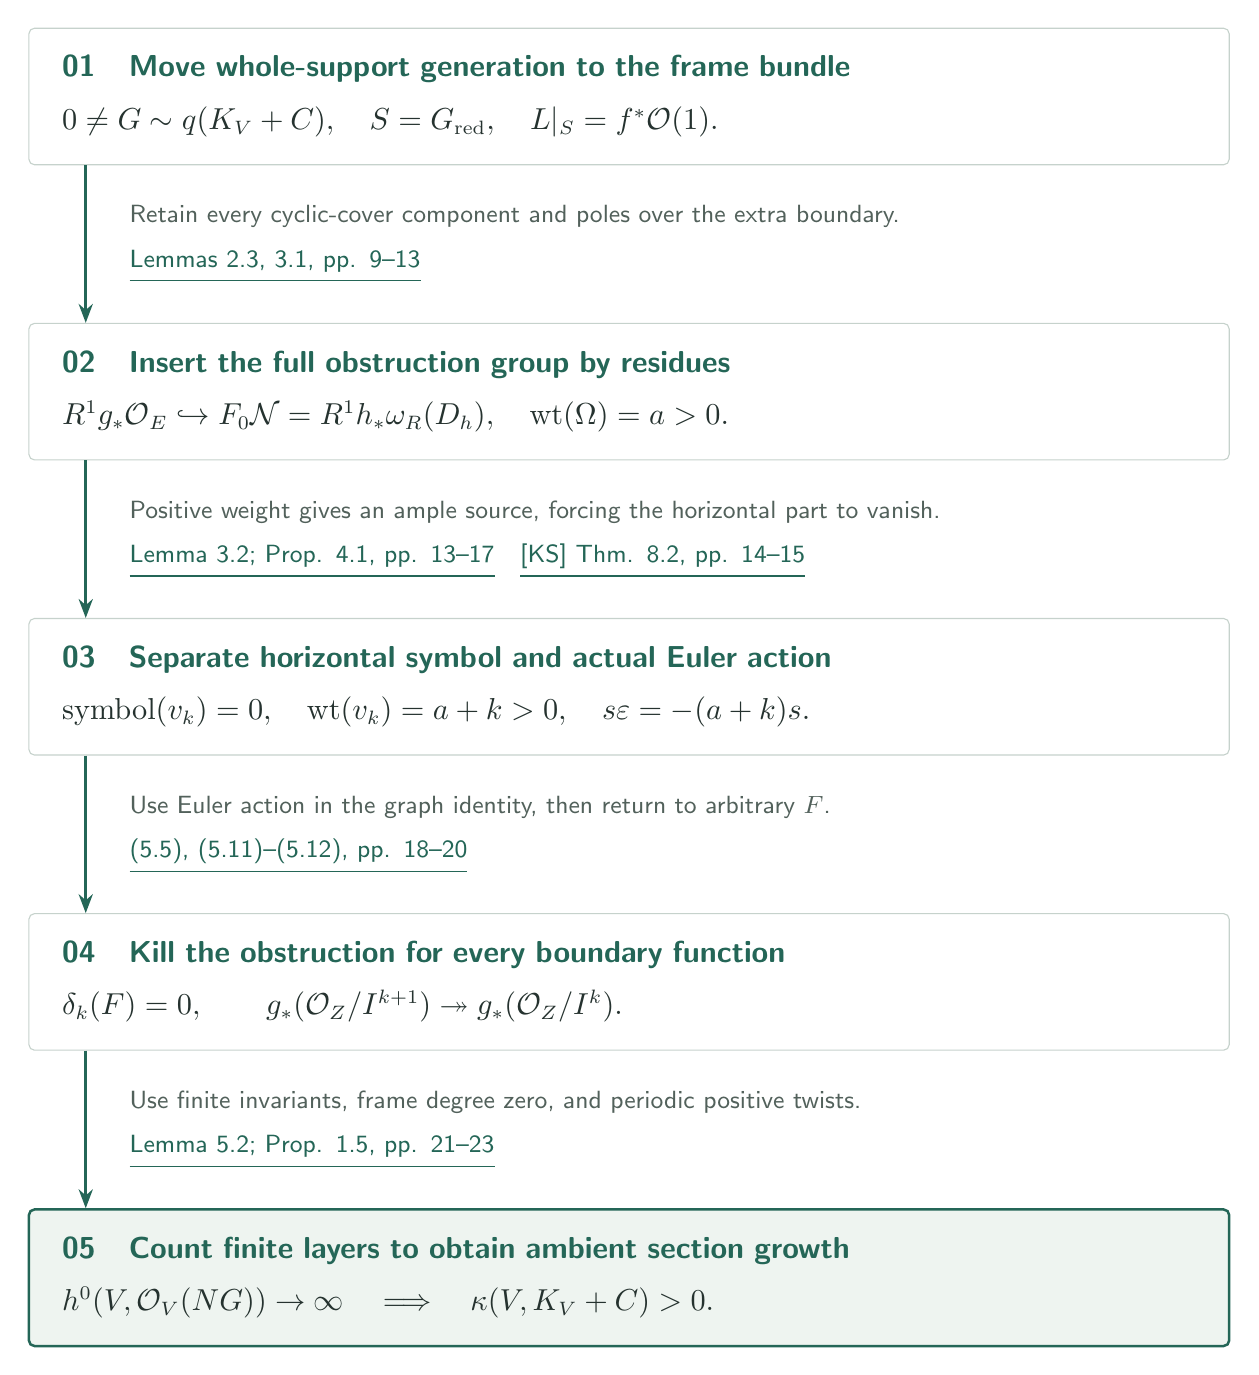
\begin{tikzpicture}
\node[card] (n0) {\heading{01}{全被約台の生成性を frame 上へ移す}{Move whole-support generation to the frame bundle}$0\ne G\sim q(K_V+C),\quad S=G_{\rm red},\quad L|_S=f^*\mathcal O(1).$};
\node[card,below=2.0cm of n0] (n1) {\heading{02}{全障害群を留数で単射に入れる}{Insert the full obstruction group by residues}$R^1g_*\mathcal O_E\hookrightarrow F_0\mathcal N=R^1h_*\omega_R(D_h),\quad\operatorname{wt}(\Omega)=a>0.$};
\flow{n0}{n1}{\Tx{循環被覆の全成分と、余分な境界上の極を残す。}{Retain every cyclic-cover component and poles over the extra boundary.}\\[4pt]\CiteSource{S}{Lemmas 2.3, 3.1, pp. 9--13}}
\node[card,below=2.0cm of n1] (n2) {\heading{03}{水平 symbol と実際の Euler 作用を分ける}{Separate horizontal symbol and actual Euler action}$\operatorname{symbol}(v_k)=0,\quad\operatorname{wt}(v_k)=a+k>0,\quad s\varepsilon=-(a+k)s.$};
\flow{n1}{n2}{\Tx{正の重みが ample な始域を作り、水平部分を消す。}{Positive weight gives an ample source, forcing the horizontal part to vanish.}\\[4pt]\CiteSource{S}{Lemma 3.2; Prop. 4.1, pp. 13--17}\quad \CiteSource{KS}{[KS] Thm. 8.2, pp. 14--15}}
\node[card,below=2.0cm of n2] (n3) {\heading{04}{任意の境界関数の障害を消す}{Kill the obstruction for every boundary function}$\delta_k(F)=0,\qquad g_*(\mathcal O_Z/I^{k+1})\twoheadrightarrow g_*(\mathcal O_Z/I^k).$};
\flow{n2}{n3}{\Tx{graph 恒等式に Euler 作用を代入し、任意の $F$ に戻る。}{Use Euler action in the graph identity, then return to arbitrary $F$.}\\[4pt]\CiteSource{S}{(5.5), (5.11)--(5.12), pp. 18--20}}
\node[result,below=2.0cm of n3] (n4) {\heading{05}{有限層を数えて周囲の切断を増やす}{Count finite layers to obtain ambient section growth}$h^0(V,\mathcal O_V(NG))\to\infty\quad\Longrightarrow\quad\kappa(V,K_V+C)>0.$};
\flow{n3}{n4}{\Tx{有限群不変部・frame 次数0・正の twist の周期性を使う。}{Use finite invariants, frame degree zero, and periodic positive twists.}\\[4pt]\CiteSource{S}{Lemma 5.2; Prop. 1.5, pp. 21--23}}
\end{tikzpicture}
\end{document}
